À présent que la stabilité des deux méthodes ImEx ont été comparées au \textit{splitting} d'opérateur, 
il est naturel de poursuivre par une expérience numérique pour qualifier la convergence de chaque méthode et 
d'évaluer la pertinence des méthodes ImEx face au \textit{splitting}.
\subsubsection{Expérience sur l'équation de Nagumo}
    \paragraph{Présentation de l'expérience}
    L'expérience est réalisée sur l'équation de Nagumo 1D à partir d'une solution initiale correspondant au profil de l'onde propagative de l'équation (voir \ref{par:analyser_operateurs_nagumo}).
    Succinctement, la simulation à lieu sur le domaine spatial $[-20,+20]$ entre $t=0$ et $t=3$.
    La grille spatial est divisée en $2^{13}$ cellules ce qui équivaut à un pas d'espace $\Delta t \approx 4.8 \, 10^{-3}$.
    Des conditions de Neumann homogènes et une vitesse de propagation adaptées permettent de maintenir le front d'onde au centre du domaine et 
    de négliger les effets de bords afin de comparer à la solution analytique exacte d'onde propagative. Les erreurs sont calculés sur le domaine $[-5,+5]$ pour ce centrer sur l'étude du front d'onde.
    \paragraph{Résultats}
    Les résultats de l'expérience sont présentés en \ref{fig:imex_vs_splitting}. Il apparaît que si le schéma de splitting et ImEx222 ont des performances similaires
    \begin{figure}[ht!]
        \centering
        \begin{subfigure}{\textwidth}
            \centering
            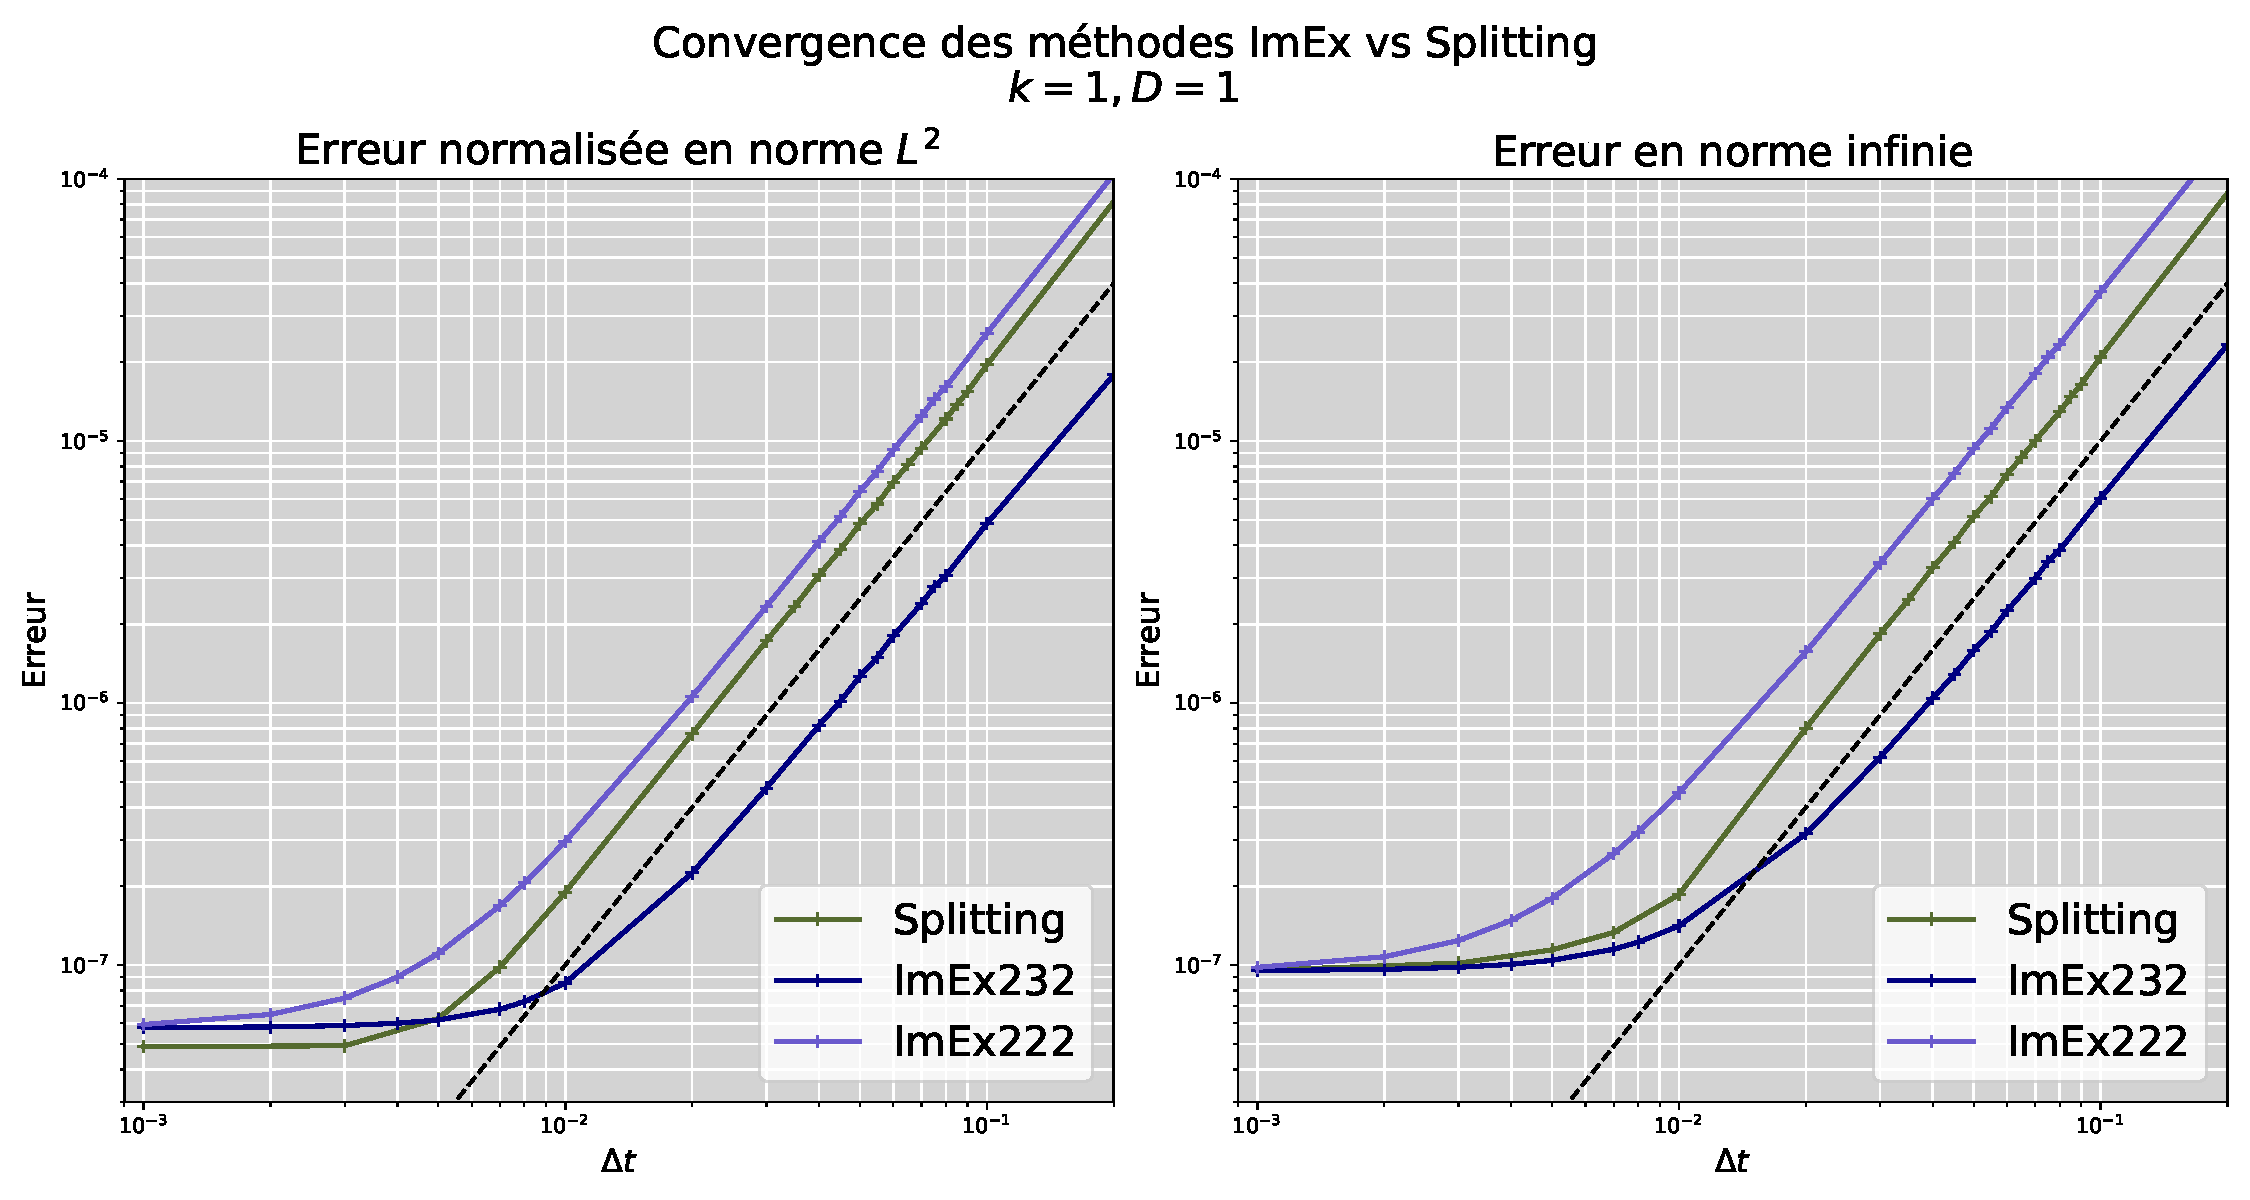
\includegraphics[width=\linewidth]{media/4_travail/2_nagumo/convergence/ImEx_vs_splitting_k1_D1.pdf}
            \caption{} % légende à compléter
            \label{fig:imex_k1_d1}
        \end{subfigure}
    \begin{subfigure}{\textwidth}
        \centering
        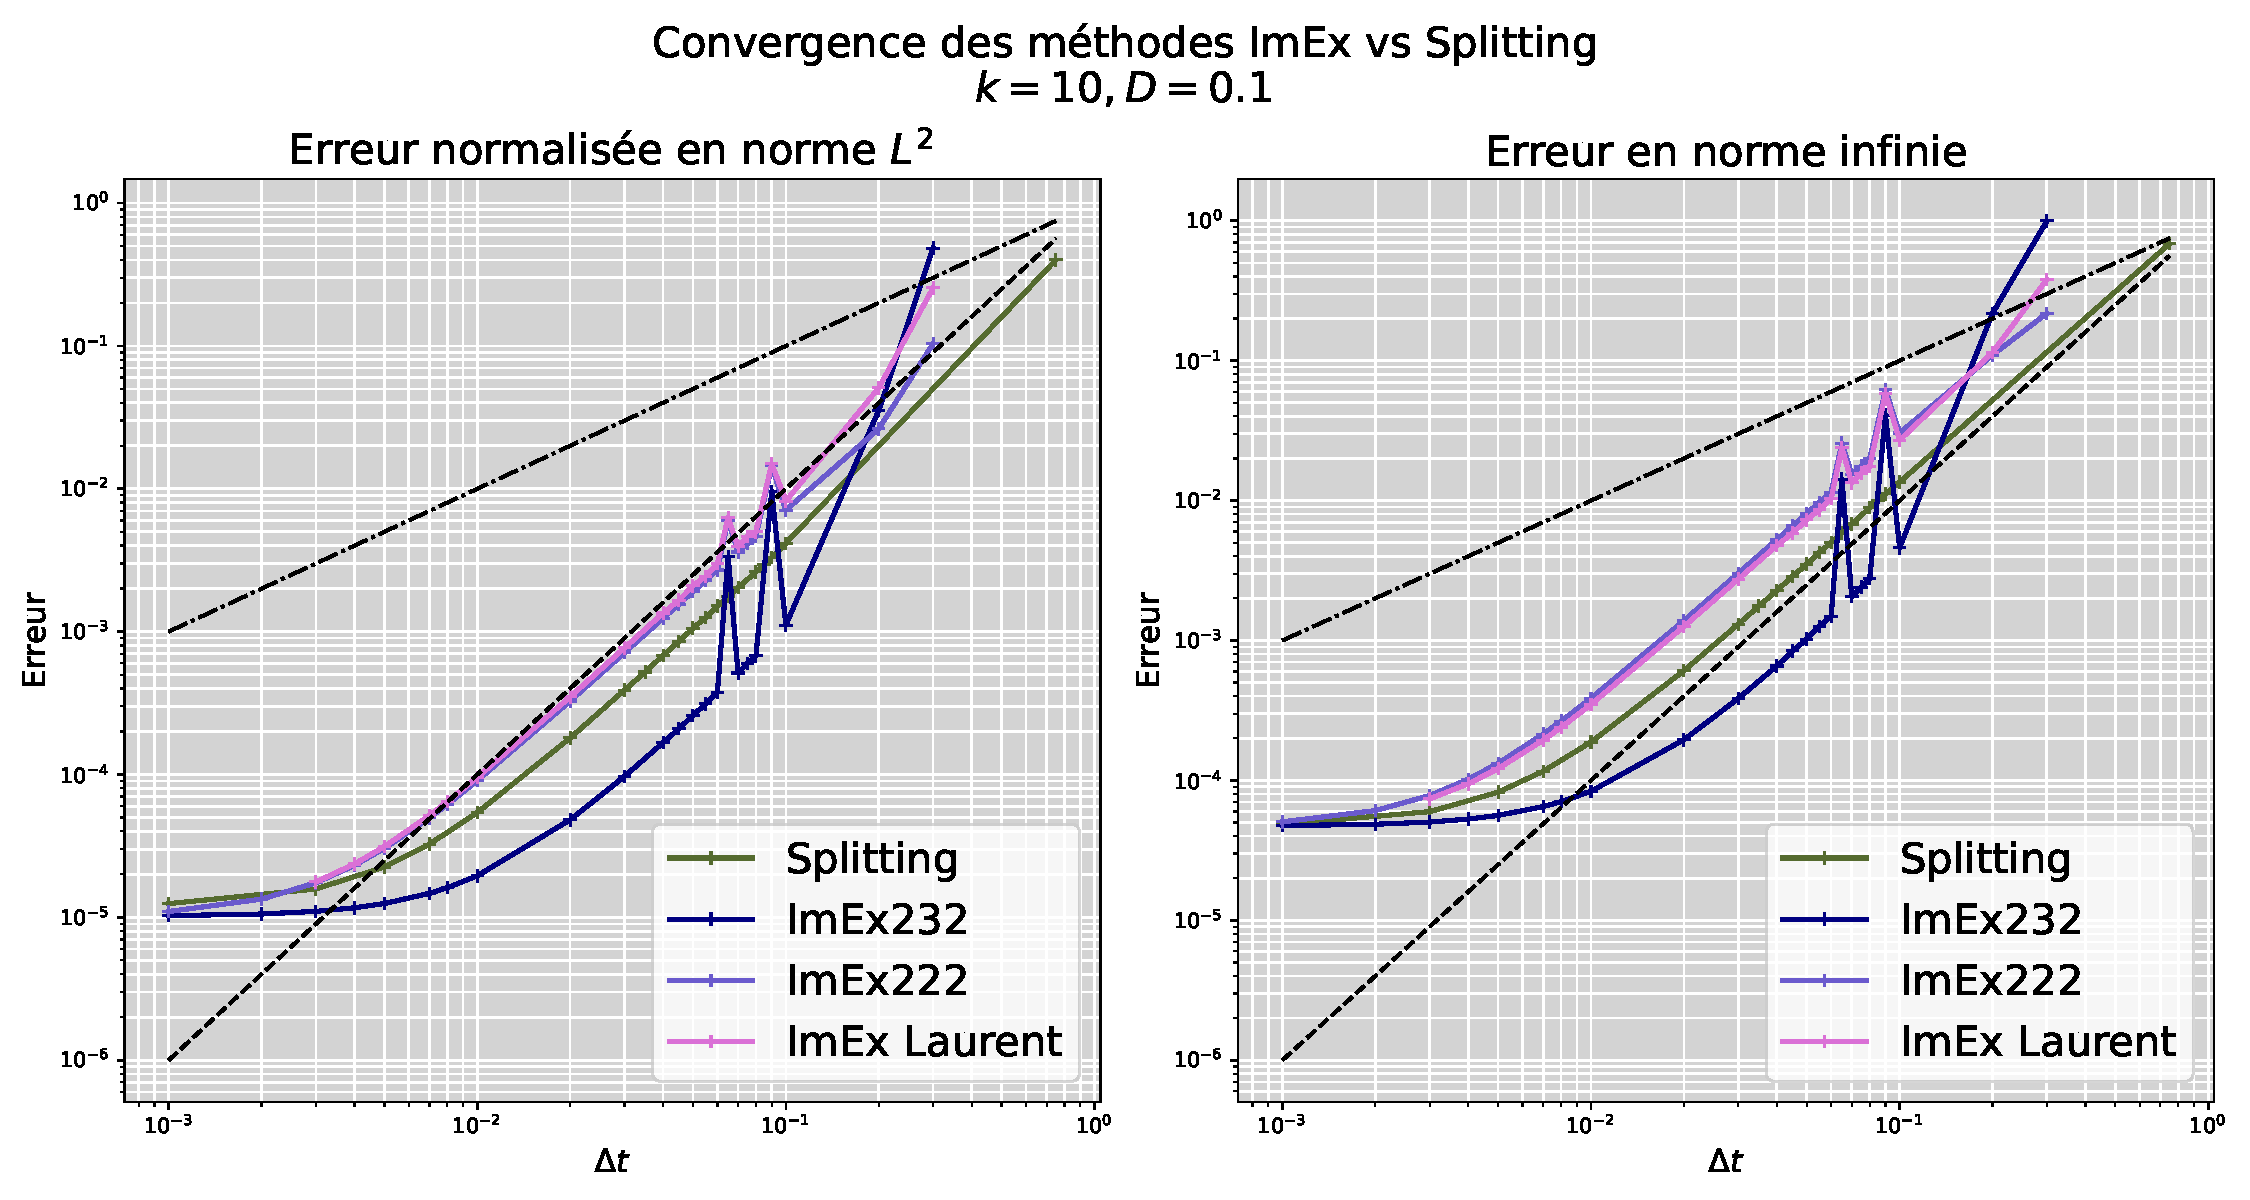
\includegraphics[width=\linewidth]{media/4_travail/2_nagumo/convergence/ImEx_vs_splitting_k10_D0.1.pdf}
        \caption{} % légende à compléter
        \label{fig:imex_k10_d01}
    \end{subfigure}
    \caption{} % légende globale de la figure
    \label{fig:imex_vs_splitting}
    \end{figure}
\newpage
\subsection{Mise en lumière expérimental de couplages entre la méthode en temps et l'adaptation spatiale}
\label{par:couplage_temps_adaptation}
L'objectif est d'observer d'éventuelles interactions entre la méthode de découplage des opérateurs (ImEx/splitting) et l'adaptation en espace par multi-résolution adaptative.
Pour ce faire la comparaison entre ImEx222, ImEx2332 et splitting a été refaite (fig \ref{fig:couplage-MRA-temps}) en adaptant spatialement chaque schéma par MRA.
Si des différences par rapport à l'étude précédente (fig. \ref{fig:imex_vs_splitting}) apparaissent, ils résultent nécessairement de couplages entre la méthode d'intégration en temps
et l'adaptation spatiale.
\begin{figure}[htbp!]
    \centering
    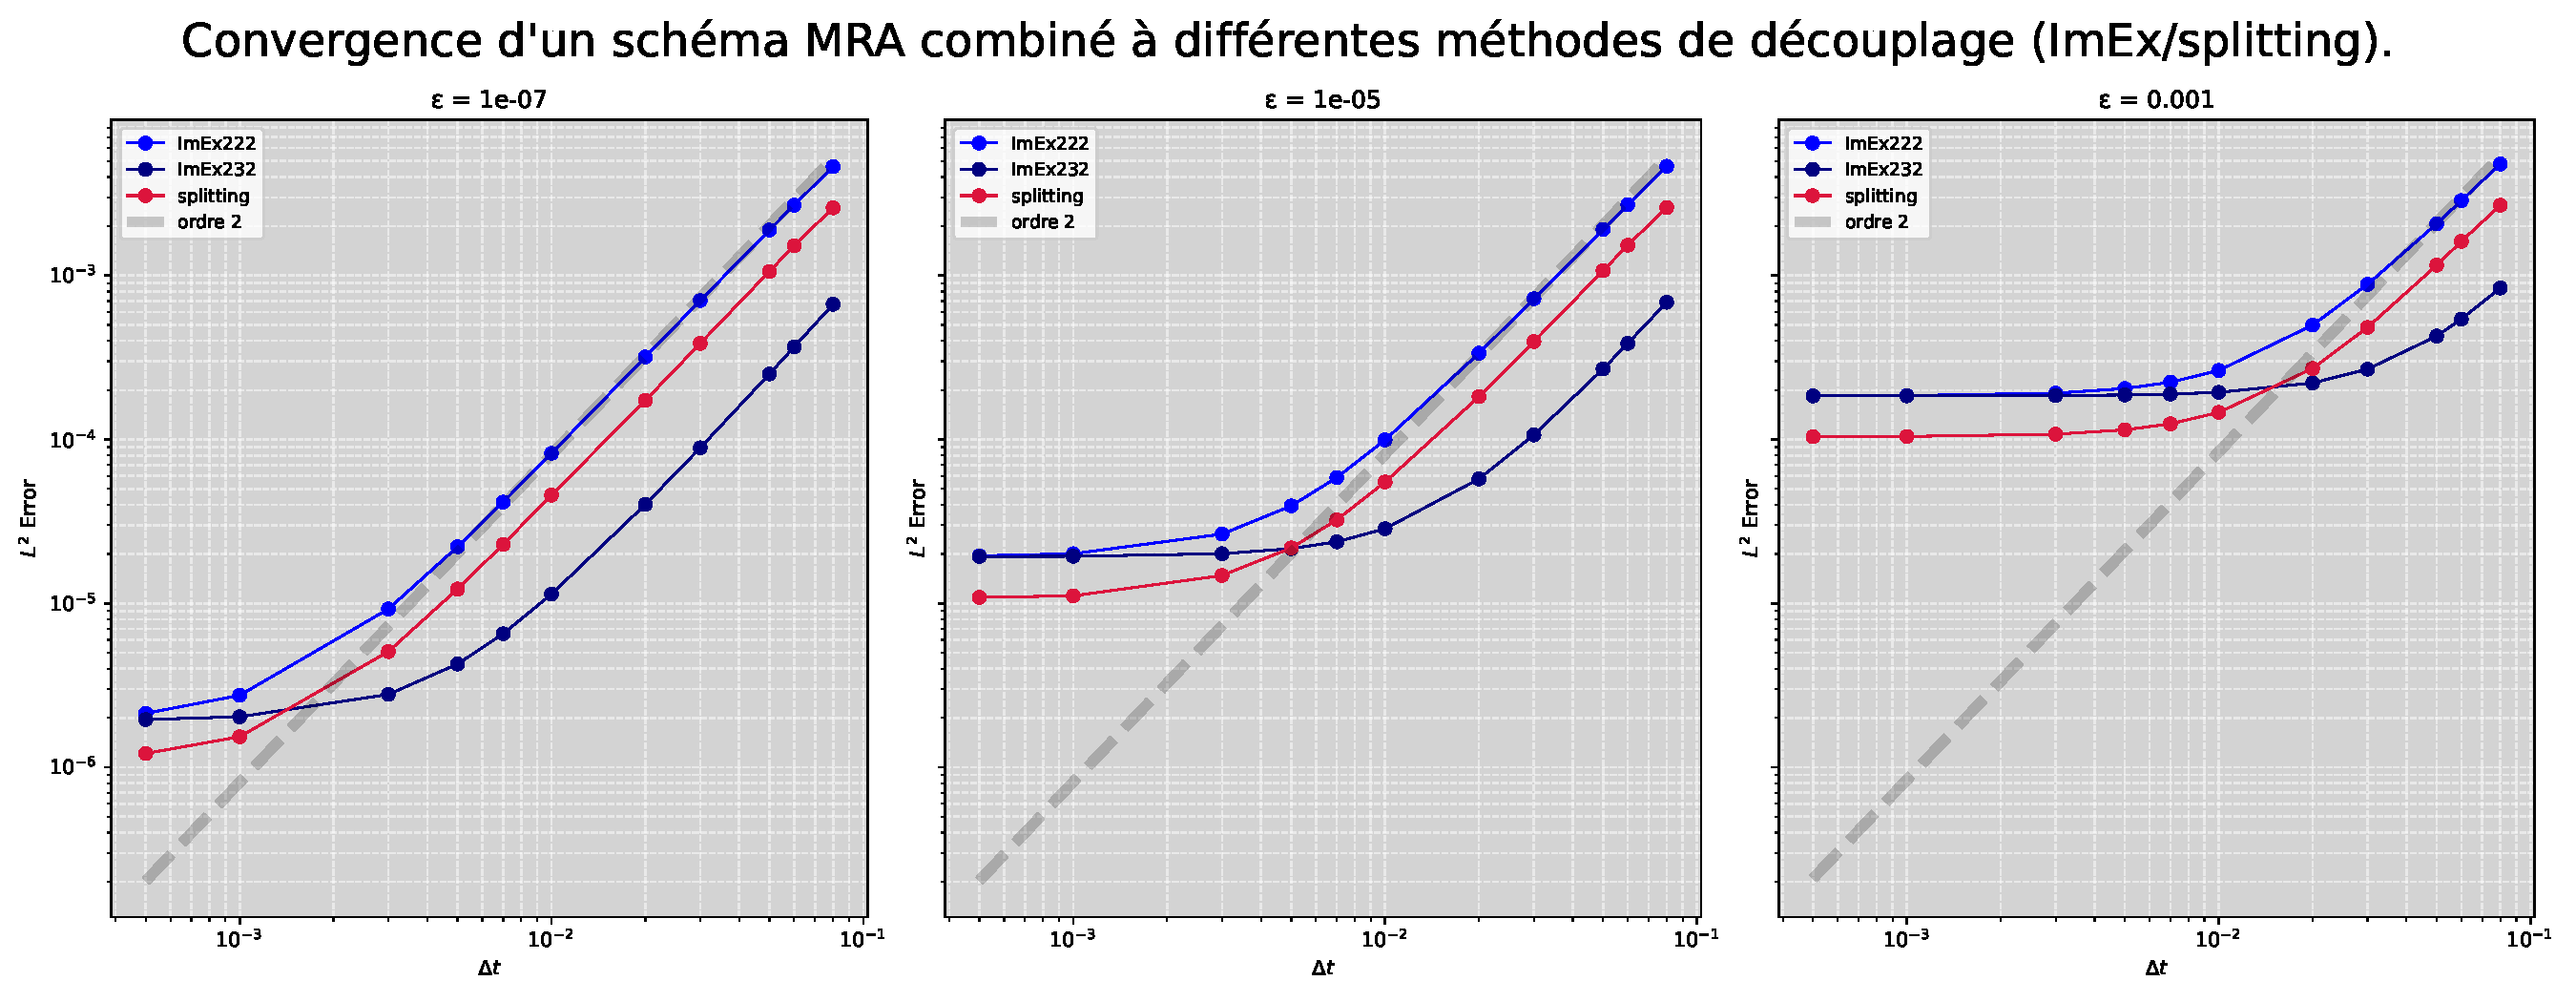
\includegraphics[width=\linewidth]{media/4_travail/2_nagumo/couplage/couplage_MRA_temps.pdf}
    \caption{Convergence des schémas ImEx et de splitting, adaptés en espace par MRA, sur l'équation de Nagumo pour $k=10$, $D=0.1$.
    Les flux sont évalués au niveau courant (pour la distinction voir \ref{par:contrib_2}), la prédiction/reconstruction est assurée par un prédicteur à trois points et l'erreur est comparé à une méthode convergé en temps.}
    \label{fig:couplage-MRA-temps}
\end{figure}
\textbf{Analyse des résultats:} pour les grands pas de temps, la convergence est similaire au cas non-adapté (fig. \ref{fig:imex_vs_splitting}). En particulier la méthode
ImEx232 exhibe une constante de convergence plus faible que le splitting. 
En revanche, lorsque l'erreur sature les méthodes ImEx offrent systématiquement des performances moins bonnes que le splitting.
La solution est comparée à une méthode quasi-exacte en temps, la convergence s'infléchie donc lorsque les erreurs de liée à la MRA sont de l'ordre des erreurs en temps.
Il semble donc que l'erreur plateau soit composée d'un terme lié à la compression, au $\varepsilon$ choisit, et d'une erreur de couplage entre l'adaptation spatiale
et la méthode en temps. Plus précisément il apparaît que les méthodes ImEx interagissent avec l'adaptation spatiale d'une manière plus néfaste que le splitting.\\
% \textbf{Limites de l'étude:} ces résultats expérimentaux peuvent être impactés par de nombreux paramètres numériques. Par exemple,
% il n'est pas garantis que les résultats soient les mêmes pour un prédicteur à 5 points au lieu de 3.